%%%%%%%%%%%%%%%%%%%%%%%%%%%%%
%% Styles, packages and new commands
\input{../Main/ML_Main.tex}
%%%%%%%%%%%%%%%%%%%%%%%%%%%%%
%% Edit the title page
\title{Machine Learning}
\subtitle{Module 1: Introduction}
\author[MOB]{Marc-Olivier Boldi}
\institute[HEC MSc Mgt BA]{Master in Management, Business Analytics, HEC UNIL}
\date{Spring 2025}
%%%%%%%%%%%%%%%%%%%%%%%%%%%%%
%%%%%%%%%%%%%%%%%%%%%%%%%%%%%
%%%%%%%%%%%%%%%%%%%%%%%%%%%%%
%%%%%%%%%%%%%%%%%%%%%%%%%%%%%
\begin{document}
%%%%%%%%%%%%%%%%%%%%%%%%%%%%%
\begin{frame}
	\titlepage
\end{frame}
%%%%%%%%%%%%%%%%%%%%%%%%%%%%%
\begin{frame}
\frametitle{Table of Contents}
	\tableofcontents
\end{frame}
%%%%%%%%%%%%%%%%%%%%%%%%%%%%%
\section{What is Machine Learning?}
%%%%%%%%%%%%%%%%%%%%%%%%%%%%%
\begin{frame}
\frametitle{What is Machine Learning?}
{\bf Machine learning} is a set of techniques using models that are trained on data to achieve forecasting or pattern discovery. 

\begin{itemize}
\item Unlike programming, consisting of implementing a solution already defined by the developers, ML let the model learn by seeing data (learning from examples). 
\item ML is a sub-field of Artificial Intelligence (AI).
\item Deep Learning is a popular sub-field of of ML that uses deep neural networks, a particular type models.
\end{itemize}
\end{frame}
%%%%%%%%%%%%%%%%%%%%%%%%%%%%%
\begin{frame}
\frametitle{Informal expectations from ML}
\begin{itemize}
\item Provide predictions and/or decisions (predictive analytics).
\item Fairly automatic and data based (not judgmental).
\item The prediction quality can be assessed (metrics).
\item The model improves with the increase/improvement of the data base.
\item The model is interpretable.
\end{itemize}
\end{frame}
%%%%%%%%%%%%%%%%%%%%%%%%%%%%%
\begin{frame}
\frametitle{Machine Learning versus Statistics}
ML is not a re-branding of statistics. Both use data and statistical models. Applications of ML are oriented toward predictions, applications of statistics are oriented toward inference (research, hypothesis assessment). E.g.,
\begin{itemize}
\item A study aims to (in)validate that employees with a psychological support are less prone to burnout. This study needs observations, data analysis, and statistical tests of hypotheses. This is typical of academic work and is usually qualified as {\it statistics} (inference).
\item A study aims to develop a prediction tool for the credit risk associated to a client in a bank. This study needs observations, data analysis, and model validation. It is typical of ML.
\end{itemize}
\end{frame}
%%%%%%%%%%%%%%%%%%%%%%%%%%%%%
\section{Data}
%%%%%%%%%%%%%%%%%%%%%%%%%%%%%
\begin{frame}
\frametitle{Data types}
Various types of data can be used in ML (non-exhaustive):
\begin{itemize}
\item {\bf Tabular data}: values organized in columns. The most common.
\item {\bf Time series}: values observed in a specific order.
\item {\bf Textual data}: words, set of words, texts, etc.
\item {\bf Image data}: e.g., $512\times 512$ pixels consisting of $3 \times$ values between 0 and 255, for a RGB color image. 
\item {\bf Video}: set of ordered images often going with sounds (coded with times series).
\item {\bf Networks and relational data}: links and distances between units (interactions in a social networks, roads on a map, etc.).
\end{itemize}
In this course, we see ML for tabular data.
\end{frame}
%%%%%%%%%%%%%%%%%%%%%%%%%%%%%
\begin{frame}
\frametitle{Data types for tabular data}
Values organized in columns. Values can be:
\begin{enumerate}
\item {\bf Categorical}: can take a finite number of predefined levels.
\begin{enumerate}
\item {\bf Nominal}: levels are unstructured. E.g., hair colors, genders, food preferences, etc.
\item {\bf Ordinal}: levels have a predefined order. E.g., $S<M<L$, Disagree $<$ Neutral $<$ Agree.
\end{enumerate} 
\item {\bf Numerical}: 
\begin{enumerate}
\item {\bf Continuous}: numbers with decimal. E.g., revenues, age, height, etc.
\item {\bf Discrete}: integers. E.g., counting people waiting in line, number of cars per household, etc. 
\end{enumerate}
\end{enumerate}
\end{frame}
%%%%%%%%%%%%%%%%%%%%%%%%%%%%%
\begin{frame}
\frametitle{Data types for tabular data}
Some data can be represented in different types or transformed. E.g., 
\begin{itemize}
\item Categorizing the revenue into an ordinal variable (intervals: $]0,10]$, $]10,20]$, etc.).
\item Assign numbers to ordinal levels. E.g., coding Likert scale, Sizes $XS=1, \ldots, XL=5$.
\item Create dummy variables for nominal variables (see later).
\end{itemize}
\end{frame}
%%%%%%%%%%%%%%%%%%%%%%%%%%%%%
\begin{frame}
\frametitle{Tabular data structure}
The table is organized as 
\begin{itemize}
\item Each row is an {\bf instance}: the unit of observation. 
\item Each column is a {\bf feature}: the variables along which the unit is measured.
\end{itemize}
Synonyms:
\begin{itemize}
\item Instances, cases, observational units... 
\item Features, variables, attributes, predictors...
\end{itemize}
\end{frame}
%%%%%%%%%%%%%%%%%%%%%%%%%%%%%
\section{Learning tasks}
%%%%%%%%%%%%%%%%%%%%%%%%%%%%%
\begin{frame}
\frametitle{Supervised and unsupervised learning}
In ML, two main tasks are addressed 
\begin{enumerate}
\item {\bf Supervised Learning} The aim is to predict an outcome of interest $y$ using features $x$. It includes regression and classification tasks, scoring, model selection, etc.  
\item {\bf Unsupervised Learning} The aim is to learn the dependence patterns of several features and to find meaningful representations of these patterns. This includes clustering and dimension reduction.
\end{enumerate}
\end{frame}
%%%%%%%%%%%%%%%%%%%%%%%%%%%%%
\begin{frame}
\frametitle{Supervised and unsupervised learning}
Examples:
\begin{enumerate}
\item {\bf Supervised Learning} A retailer wants to forecast the spending of a category of customers in reaction to a marketing campaign. 
\item {\bf Unsupervised Learning} A retailer wants to group customers in different profiles according to what they buy and their personal characteristics. The profiles are not known in advance.
\end{enumerate}
\end{frame}
%%%%%%%%%%%%%%%%%%%%%%%%%%%%%
\begin{frame}
\frametitle{Supervised learning tasks and the outcome}
For supervised learning, one (or several) feature has a specific interest because it is to be predicted using the other features. It is called the {\bf outcome} (syn. the response).\\
\vspace{0.3cm}
Two types of sub-tasks are distinguished depending on the outcome:
\begin{itemize}
\item {\bf Classification}: the outcome is categorical.
\begin{itemize}
\item A binary outcome: {\bf binary} classification
\item More than two levels: {\bf multi-class} classification 
\end{itemize}
\item {\bf Regression}: the outcome is numerical.
\end{itemize}
{\it Note:} regression task and regression (e.g., linear model) are not the same thing. Regressions can used for the regression task but (a lot of) other models exist. 
\end{frame}
%%%%%%%%%%%%%%%%%%%%%%%%%%%%%
\begin{frame}
\frametitle{Example of a Machine Learning task}
Bank customers (instances) are predicted
\begin{itemize}
\item Outcome: credit risk (Good/Bad),
\item Attributes (features):
\begin{itemize}
\item Status of existing checking account, 
\item Duration in month,
\item Credit history,
\item etc.
\end{itemize}
\end{itemize}
\scriptsize
See {\url https://archive.ics.uci.edu/ml/datasets/statlog+(german+credit+data)}\\
\normalsize
\vspace{0.3cm}
What task is it?
\end{frame}
%%%%%%%%%%%%%%%%%%%%%%%%%%%%%
\section{Models}
%%%%%%%%%%%%%%%%%%%%%%%%%%%%%
\begin{frame}
\frametitle{Models}
Supervised learning has two pillars: the data and the models.\\
\vspace{0.3cm}
A {\bf model} is a trainable algorithm which takes features $x$ and returns an output $\hat{y}$, a prediction of the outcome $y$ corresponding to $x$.
\begin{center}
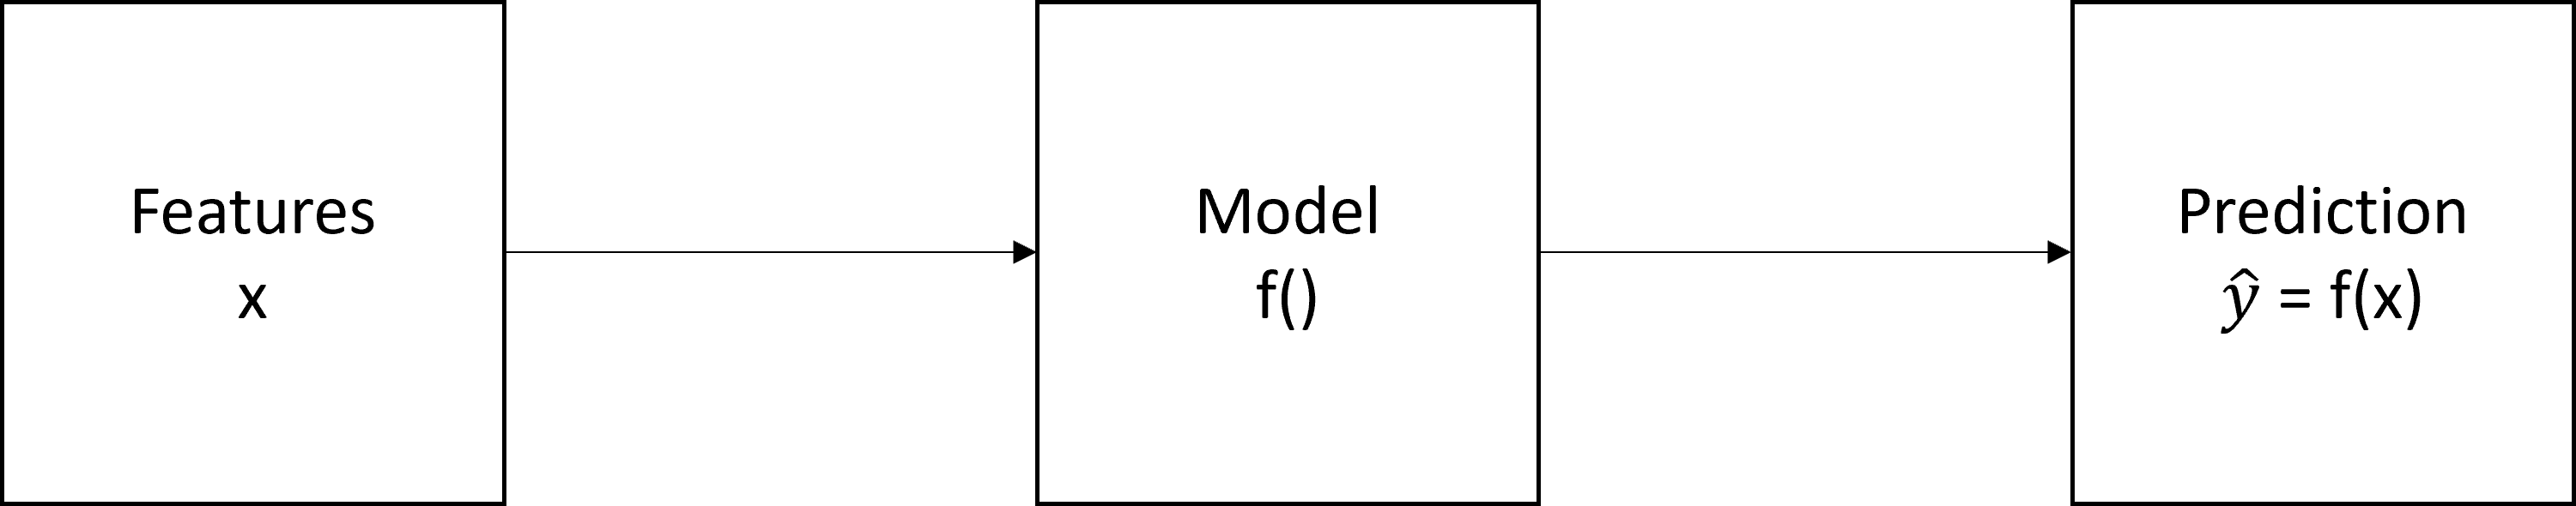
\includegraphics[width=10cm]{../Graphs/ML1.png}
\end{center}
Synonyms: {\bf learners}, {\bf algorithms}. For classification, {\bf classifiers}. \\
\vspace{0.3cm}
Notations: $f(\cdot)$ is the model and $\hat{y} = f(x)$ is the prediction at $x$.
\end{frame}
%%%%%%%%%%%%%%%%%%%%%%%%%%%%%
\begin{frame}
\frametitle{Model training}
The model is {\bf trainable}. It can be trained to the available data to produce good predictions.\\
\vspace{0.3cm}
The model, which is itself an algorithm, comes with a training algorithm that can adapt the parameters of the model to optimize a quality criterion. The training algorithm is specific to the model and the criterion. For a given model, you may have several choices (several criteria, several training algorithms, etc.).
\end{frame}
%%%%%%%%%%%%%%%%%%%%%%%%%%%%%
\begin{frame}
\frametitle{Model training: example}
We want to predict $y$ from features $x$ with a linear regression. This model has parameters $\beta$. Training the model to the data means selecting $\beta$ from the $(y_i,x_i)$, $i=1,\ldots,n$. Below are two possible criteria:
\begin{enumerate}
\item The mean square of the errors (MSE). The optimal parameter $\hat{\beta}$ is called the Ordinary Least Square (OLS) 
$$
\hat{\beta} = \arg\min_\beta \frac{1}{n}\sum_{i=1}^n (y_i - x_i^T \beta)^2.
$$
\item The L1-penalized MSE. The optimal parameter $\hat{\beta}$ is the LASSO (least absolute shrinkage and selection operator) 
$$
\hat{\beta} = \arg\min_\beta \frac{1}{n}\sum_{i=1}^n (y_i - x_i^T \beta)^2 + \lambda \Vert \beta\Vert_1
$$
\end{enumerate}
\end{frame}
%%%%%%%%%%%%%%%%%%%%%%%%%%%%%
\begin{frame}
\frametitle{Model training: optimization}
In general, each criterion leads to a different set of parameters and a different model. No one is uniformly better than the others. E.g., the OLS has a smaller MSE on the training data (better fit) but the LASSO is more robust against overfitting. It however comes at the cost of selecting $\lambda$. \\ 
\vspace{0.3cm}
Depending on the model, it can have several options for its training. It requires the {\it minimization} (resp. {\it maximization}) of a {\bf loss} (resp. {\bf goodness-of-fit}) function. It is {\bf always data based}. \\
\vspace{0.3cm}
How the optimization is done is part of the so-called {\bf black box} aspect of machine learning models: people don't know what is going on with the mathematics put in action when pushing the training button.\\
\vspace{0.3cm}
Fortunately, in this course, we will study some of these optimizations for some models.
\end{frame}
%%%%%%%%%%%%%%%%%%%%%%%%%%%%%
\section{Metrics}
%%%%%%%%%%%%%%%%%%%%%%%%%%%%%
\begin{frame}
\frametitle{Metrics}
After training, we have the best version of a model for the data, according to the chosen criterion. Is it the best model? Is it just doing a good job? To answer, we use {\bf metrics}: the quality of the model predictions: 
\begin{itemize}
\item Classification: accuracy, specificity, sensitivity, balanced accuracy, $F1$, entropy, etc.
\item Regression: $R^2$, RMSE, MAE, etc.
\end{itemize}
Interpreting or comparing these metrics allows to evaluate the model performance.\\
\vspace{0.3cm}
A fundamental aspect of metrics is that {\bf they are only based on the predictions and the data}. Thus, different models can be compared.
\end{frame}
%%%%%%%%%%%%%%%%%%%%%%%%%%%%%
\begin{frame}
\frametitle{Model selection}
A classical approach in ML consists of putting several models in competition. These cross-model comparisons are achieved comparing their metrics: the best model is the one achieving the best metric.\\
\vspace{0.3cm}
E.g., you want to build a predictor for real estate prices from observable features ($m^2$, location, type, etc.). You train one linear regression with OLS, one linear regression with LASSO, one regression tree, one neural network, etc. You select the model with the lowest MSE on unseen data set aside before the training. \\
\vspace{0.3cm}
This is possible only because (again) {\bf the metrics are only based on the predictions and the data} so that models with different constructions and intrinsic characteristics can be compared. 
\end{frame}
%%%%%%%%%%%%%%%%%%%%%%%%%%%%%
\begin{frame}
\frametitle{Base model}
It is a good practice to have a {\bf base model} to get a reference whether a final is worthy or not.\\
\vspace{0.3cm} 
E.g., for the prediction of the real estate price, the base model could be the linear regression with OLS since this model is common. Suppose at the end of the selection, you select the neural network with an MSE improved by $1\%$ compared to the OLS regression.\\ 
\vspace{0.3cm}
Is it worth using a complex neural network, heavy to manipulate, not transparent, and energy consuming for such a small improvement~?
\end{frame}
%%%%%%%%%%%%%%%%%%%%%%%%%%%%%
\section{Overfitting}
%%%%%%%%%%%%%%%%%%%%%%%%%%%%%
\begin{frame}
\frametitle{Overfitting}
{\bf Overfitting} is one of the worst enemy in ML:
\begin{itemize}
\item A model is trained on the observed data. 
\item The predictions are used for future data.
\end{itemize}
Overfitting arises when the model is well trained on the observed data, but has a low capacity of {\bf generalization} outside this data base. 
\end{frame}
%%%%%%%%%%%%%%%%%%%%%%%%%%%%%
\begin{frame}
\frametitle{Overfitting}
E.g., for real estate price prediction, consider the silly model: 
\begin{itemize}
\item If the apartment is already in the observed data base, the predicted price is the one in the data base. 
\item If it is a new apartment, the predicted price is random. 
\end{itemize}
The MSE on the data base will be close to zero since the model predicts all observed data exactly. \\ 
\vspace{0.3cm}
However, this model is useless to the company that cannot use it for new apartments. This model "overfits" the observed data base. 
\end{frame}
%%%%%%%%%%%%%%%%%%%%%%%%%%%%%
\begin{frame}
\frametitle{Detect overfitting}
To detect overfitting, {\bf data splitting strategies} are applied: 
\begin{itemize}
\item Splitting the data base into a {\bf training set}\footnote{The training set is often further split into a ``training set'' and a ``validation set'' for the selection of the hyperparameters. This will be clarified later.} and a {\bf test set}. In the previous example, the silly model would achieve a perfect accuracy on the training set but a poor accuracy on the test set (because it never saw these data before): that difference reveals the overfitting. 
\end{itemize}
More complex strategies exist like
\begin{itemize}
\item {\bf Cross-validations}
\item {\bf Bootstrap}
\end{itemize}
\end{frame}
%%%%%%%%%%%%%%%%%%%%%%%%%%%%%
\begin{frame}
\frametitle{Avoid overfitting}
Data splitting is useful to select one model among several to avoid overfitting. However, if all the models are prompt to overfit, data splitting will not help. \\
\vspace{0.3cm}
Overfitting often results from too much complexity in the model. Complexity arises when the model has a lot of parameters. Avoiding overfitting can be obtained by constraining the model to less parameters, i.e., less complexity.\\ 
\vspace{0.3cm}
When a model is trained, {\bf goodness-of-fit} and {\bf complexity} are taken into account. A complex model is prompt to overfit while a too simple model will be prompt to under-fit. The trained model should satisfy a {\bf compromise} between these two.\\
\vspace{0.3cm}
E.g., LASSO is a constrained OLS that penalizes the complexity by shrinking toward $0$ some of the components of $\beta$.
\end{frame}
%%%%%%%%%%%%%%%%%%%%%%%%%%%%%
\section{Interpretation}
%%%%%%%%%%%%%%%%%%%%%%%%%%%%%
\begin{frame}
\frametitle{Interpretation}
ML models can be {\bf black boxes}, i.e., they are difficult to interpret. Interpretation in ML consists in 
\begin{itemize}
\item Discover {\bf if} a feature (variable) is important for the prediction of the outcome. E.g., what influences the price of an apartment\footnote{Caution: link, association, correlation $\neq$ causality!!} according to the model~?
\item Discover {\bf how} the feature is related to the outcome. E.g., Does the price increase when you move away from the city center?
\end{itemize}
Several techniques exist (see later).\\
\vspace{0.3cm} 
Interpretation is often an aim in itself for ML (more important than the prediction task itself). 
\end{frame}
%%%%%%%%%%%%%%%%%%%%%%%%%%%%%
\begin{frame}
\frametitle{Supervised learning steps}
\small
With training/test set splitting\\
\normalsize
\begin{center}
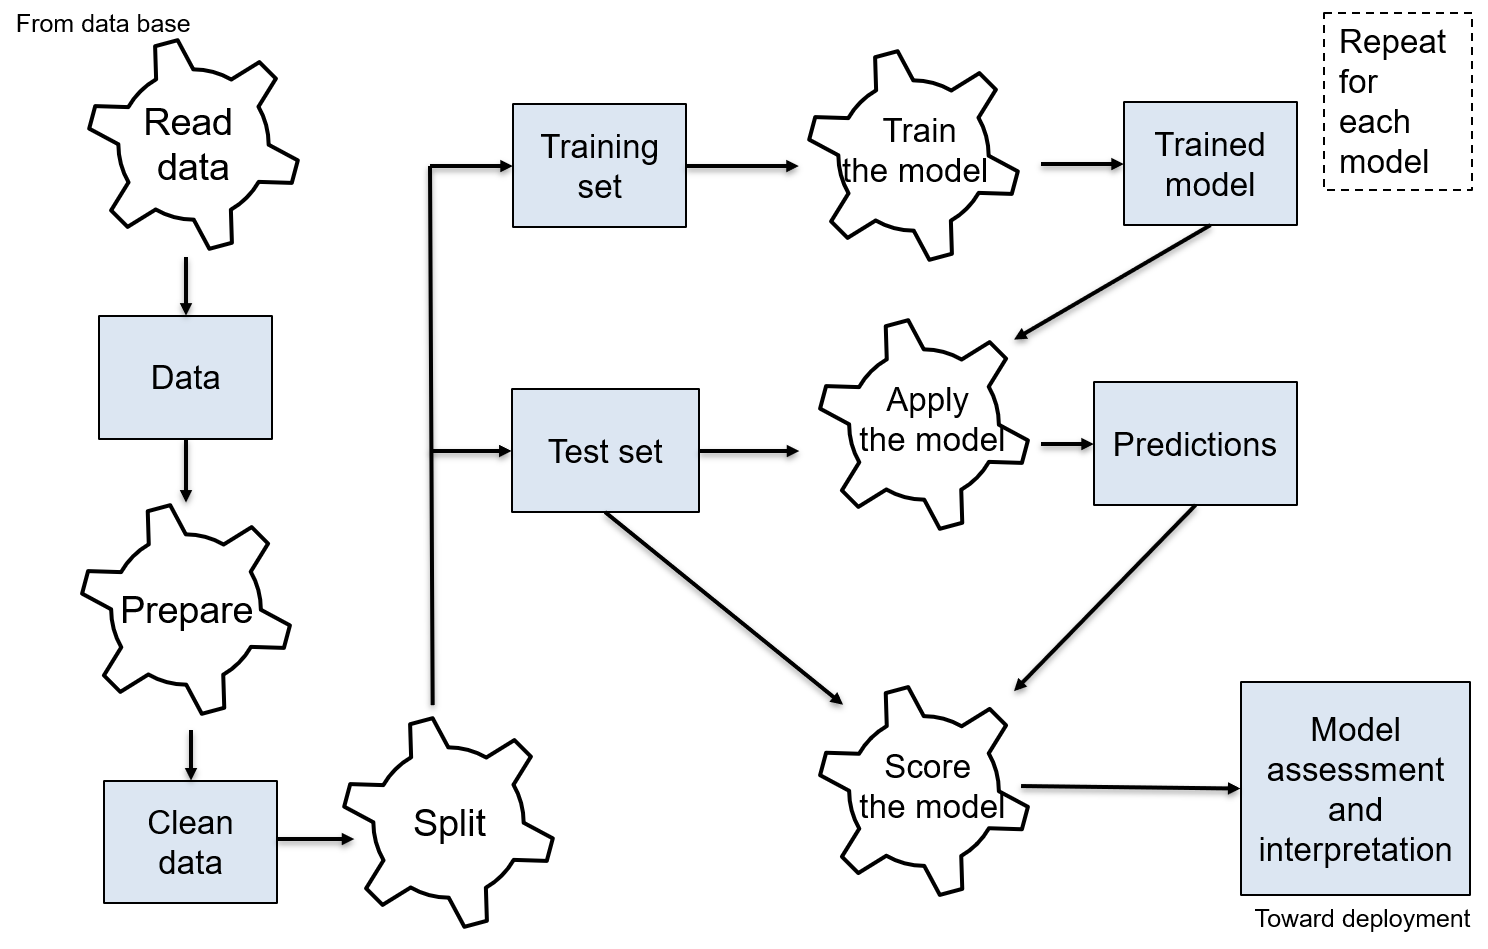
\includegraphics[width=9cm]{../Graphs/ML_steps.png}
\end{center}
\end{frame}
%%%%%%%%%%%%%%%%%%%%%%%%%%%%%
\section{Skills and tools}
%%%%%%%%%%%%%%%%%%%%%%%%%%%%%
\begin{frame}
\frametitle{Skills}
Useful skills for ML (non-exhaustive):
\begin{itemize}
\item Knowledge: ML is an active and moving field. Stay informed!
\item Programing: success factor for a ML project as developer and/or manager. 
\item Communication: not specific to ML project but the technicality of the topic makes it more complex. 
\end{itemize}
\end{frame}
%%%%%%%%%%%%%%%%%%%%%%%%%%%%%
\begin{frame}
\frametitle{Tools}
Several tools (computer programs, apps, webpages, etc.) allow to build ML solutions. In this course, we use {\tt R} and {\tt Python}:
\begin{itemize}
\item Most used programs. {\tt R} for data exploration, low and medium-level ML, and (classical) statistics; {\tt Python} for all-level ML. 
\item Open, free, and well documented (help, forums, etc.).
\item Serious, widespread, and under continuous development with an active community.
\end{itemize}
\end{frame}
%%%%%%%%%%%%%%%%%%%%%%%%%%%%%
\end{document}
